\documentclass[oneside,a4paper,14pt]{extarticle} %размер шрифта 14
\usepackage[T1,T2A]{fontenc}
\usepackage[
	a4paper,
	letterpaper,
	top=2cm,
	bottom=2cm,
	left=2.5cm,
	right=1.5cm
]{geometry} 
\usepackage[utf8]{inputenc} %кодировка текста
\usepackage[russian]{babel} %поддержка русского языка
\usepackage{textcomp} %текстовые символы
\usepackage{indentfirst} %корректировка отступов
\usepackage{graphicx} %работа с изображениям
\usepackage{minted} %
\usepackage{mwe} % for blind text and example-image-a in example
\usepackage{wrapfig}
\usepackage{caption}
\usepackage{amsmath}  % для формул и символов
\usepackage{amsfonts}
\usepackage{amsthm}
\usepackage[all]{xy}
\usepackage[breaklinks]{hyperref}
%%размер кегля у заголовков разделов 
\usepackage{titlesec} 
\titleformat{\section}
{\normalsize\bfseries} 
{\thesection} {1em}{} 
\titleformat{\subsection}
{\normalsize\bfseries}
{\thesubsection} {1em}{} 
\titleformat{\subsubsection}
{\normalsize\bfseries}
{\thesubsection} {1em}{}

\renewcommand\baselinestretch{1.33}\normalsize % межстрочный интервал
\setlength{\parindent}{1.25cm}
\usepackage{indentfirst}


\begin{document}
	\newpage\thispagestyle{empty}
	\begin{center}
		МИНИСТЕРСТВО НАУКИ И ВЫСШЕГО ОБРАЗОВАНИЯ\\
			РОССИЙСКОЙ ФЕДЕРАЦИИ
			ФЕДЕРАЛЬНОЕ ГОСУДАРСТВЕННОЕ БЮДЖЕТНОЕ\\
			ОБРАЗОВАТЕЛЬНОЕ
			УЧРЕЖДЕНИЕ ВЫСШЕГО ОБРАЗОВАНИЯ\\
			«ВЯТСКИЙ ГОСУДАРСТВЕННЫЙ УНИВЕРСИТЕТ»\\
			Институт математики и информационных систем\\
			Факультет автоматики и вычислительной техники\\
			Кафедра электронных вычислительных машин
	\end{center}
	\vspace{20mm}
	
	\begin{center}
		Отчёт по лабораторной работе №2\\
		по дисциплине\\
		<<Информатика>>\\
		% <<>>\\
	\end{center}
	\vspace{48mm}
	
	Выполнил студент гр. ИВТб-1303-06-00 \hspace{10mm} \rule[-0,5mm]{23mm}{0.15mm}\,/Гортоломей И.К./
	
	
	Проверил доцент кафедры ЭВМ \hfill  \rule[-0,5mm]{30mm}{0.15mm}\,/Коржавина А.С./
	
	\vfill
	\begin{center}
		Киров\\
		2025
	\end{center}

	\newpage%\thispagestyle{empty}
	
	\section*{Цель} 
	Цель работы: закрепить на практике лекционный материал по теме «Системы счисления», реализовав программно несколько базовых алгоритмов работы в системах счисления с произвольными основаниями.
	
	\section*{Задание}
	\begin{enumerate}
  \item Выполнить минимизацию булевых функций, представить функции различных базисах – основном логическом базисе (О), в базисе Шеффера (Ш), Пирса (П) или Жегалкина(Ж) в соответствии с вариантом, после чего построить схему в системе Logisim и выполнить проверку.
  \item Построить четырехразрядный полный сумматор, складывающий 2 двоичных четырехразрядных числа и учитывающий единицу переноса. Построить схему сумматора в Logisim, проверить его работоспособность.
  \item Построить схемы прямого (на +1) и обратного (на -1) 4-разрядных двоичных счетчиков на счетных (T) триггерах. Построить схемы счетчиков в Logisim, проверить их работоспособность.
  \item Гирлянда. На базе счетчика, дешифратора построить схему, включающие светодиоды в определенном порядке в зависимости от варианта. Построить схему в Logisim, проверить его работоспособность.
  \item Построить схему дешифратора семисегментного индикатора.
  \item Построить схему 4-разрядного последовательного сдвигового регистра.  Сдвиг в любую сторону, запись последовательная по битам, чтение параллельное.
  \item Построить схему последовательного (shift-add) 8-разрядного умножителя на сдвиговом регистре.
  \item Построить схему 64-разрядного сумматора с ускоренным переносом.
\end{enumerate}

	\newpage
	
	\section*{Решение}
	\begin{enumerate}
	\item задание. \\
	
\includegraphics[width=17cm]{1.pdf}
	\inputminted{C}{1.c}
	\newpage

	\item задание. \\
	\includegraphics[width=17cm]{2.pdf}
	\inputminted{C}{2.c}
	\newpage

	\item задание. \\
	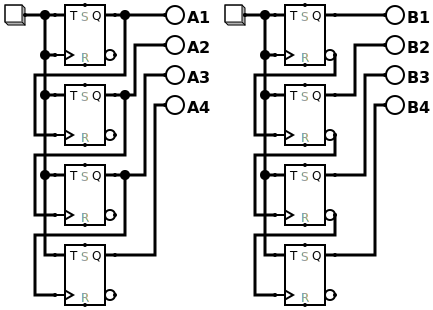
\includegraphics[width=17cm]{3.pdf}
	\newpage
	\inputminted{C}{3.c}
	\newpage

	\item задание. \\
	\includegraphics[width=17cm]{4.pdf}
	\newpage
	\inputminted{C}{4.c}
	\newpage

	\item задание. \\
	
\includegraphics[width=17cm]{5.pdf}
	\newpage
	\inputminted{C}{5.c}
	\newpage

	\item задание. \\
	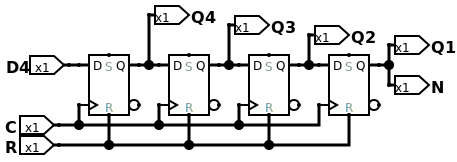
\includegraphics[width=17cm]{6.pdf}
	\newpage
	\inputminted{C}{6.c}
	\newpage

	\item задание. \\
	\includegraphics[width=17cm]{7.pdf}
	\newpage
	\inputminted{C}{7.c}
	\newpage

	\item задание. \\
	\includegraphics[width=17cm]{8.pdf}
	\newpage
	Код на Си (с двойной точностью):
	\inputminted{C}{81.c}
	Вывод: \\
	-1180591620717411303424.000000 \\
	1.172604 \\
	0.000000, 0.000000, 0.000000, 0.000000 \\
	\newpage
	Код на Паскале (с одинарной точностью):
	\inputminted{Pascal}{82.pas}
	Вывод: \\
	576460752300000000.000000 \\
	1.172604 \\
	0.000000, 0.000000, 0.000000, 0.000000 \\
	\newpage
	Код на Питоне:
	\inputminted{Python}{83.py}
	Вывод: \\
	1.1805916207174113e+21 \\
	-0.8273960599468213 \\
	0.0, 0.0, 0.0, 0.0 \\
	\newpage
\end{enumerate}

	\section*{Выводы}
	В ходе работы были успешно закреплены на практике ключевые алгоритмы работы с системами счисления.
	Реализованные программы позволяют анализировать двоичное представление чисел,
	извлекать цифры из чисел в произвольных системах счисления,
	выполнять двоичное кодирование с заданным количеством разрядов,
	осуществлять равномерное кодирование событий и преобразовывать числа в троичный симметричный код.
	
\end{document}